\section{General Theory}
\subsection{Image processing}
Image processing is a method of performing operations on an image to extract information or enhance its features. It is a broad field that covers a range of techniques, including image acquisition, Pre-processing, segmentation, feature extraction, image analysis, and visualization. In general, image processing involves transforming an image into a more useful form for analysis or display. This can be achieved through a variety of techniques, such as filtering, edge detection, Thresholding, and morphological operations. Image processing has numerous applications in various fields, including medicine, remote sensing, surveillance, robotics, and entertainment. \cite{wilhelm2016digital}, \cite{tyagi2018understanding} 

\subsection{Deep Learning and Neural Networks}
Deep learning is another name for a multilayer artificial neural network or multilayer perceptron. The elementary
bricks of deep learning are the neural networks, that are combined to form the deep neural networks.

\begin{table}[htbp]
\centering
\caption{Comparing Neural Networks and Deep Learning}
\footnotesize
\begin{tabular}{ |p{3cm}|p{5cm}|p{5cm}| }%{ |c|c|c| }
\hline
Feature & Neural Networks & Deep Learning \\
\hline
Structure & Single-layer or shallow neural networks (typically two to three layers) & Deep neural networks with multiple layers (typically more than three) \\
\hline
Learning Ability & Can learn simple patterns and make predictions & Can learn complex patterns, including abstract relationships, and make more accurate predictions \\
\hline
Data Requirements & Requires less training data & Requires more training data to learn complex patterns patterns \\
\hline
Computational Cost & Less computationally expensive & More computationally expensive, especially for deep neural networks with many layers \\
\hline
Applications & Image classification, fraud detection, spam filtering & Image recognition, natural language processing, speech recognition, medical diagnosis, self-driving cars \\
\hline
\end{tabular}
\end{table}

The term "deep" in deep learning refers to the use of multiple layers in the neural network. Deep learning models, often called deep neural networks (DNNs), are capable of learning and representing complex patterns and hierarchical features from data. \cite{nielsen2015neural} \cite{Arnold2011AnIT}, \cite{2015Natur.521..436L} \\

We have different types of deep learning systems depending upon the neural network architecture and its working principles. For example, feed-forward neural networks, convolutional networks, recurrent neural networks, autoencoders, and deep beliefs are different types of deep learning systems.
These techniques have enabled significant progress in the fields of sound and image processing, including facial recognition, speech recognition, computer
vision, automated language processing, and text classification (for example spam recognition). Potential applications are very numerous. A spectacular example is the AlphaGo program, which learned to play the go game by the deep learning method, and became the world champion in 2016.\cite{koons2005}, \cite{shinde2018review}, \cite{choi2020introduction}
\begin{figure}[H]
    \centering
    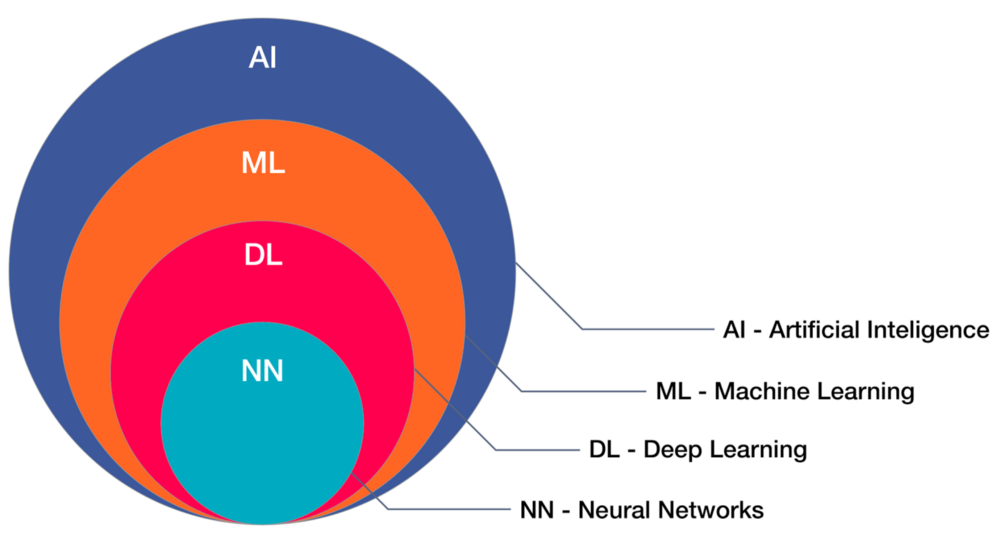
\includegraphics[width=0.8\linewidth]{tex/img/NN_DL_ML.png}
    \caption{Neural network core of deep learning \protect\href{https://intellipaat.com/community/9868/what-is-the-difference-between-deep-learning-and-traditional-artificial-neural-network-machine-learning}{\textcolor{blue}{Source}}}
    \label{fig:NN_DL}
\end{figure}

\subsection{Neural Networks}
The basic building blocks of deep learning. These networks consist of layers of interconnected nodes (neurons) that process information.
An artificial neural network (ANN) is a computing system that is designed to work the way the human brain works.

\subsubsection{The Biological Inspiration}
The brain has been extensively studied by scientists. Vast complexity prevents all but rudimentary understanding. 
- Engineers modified the neural models to make them more useful, less like biology and kept much of the terminology

\begin{figure}[H]
    \centering 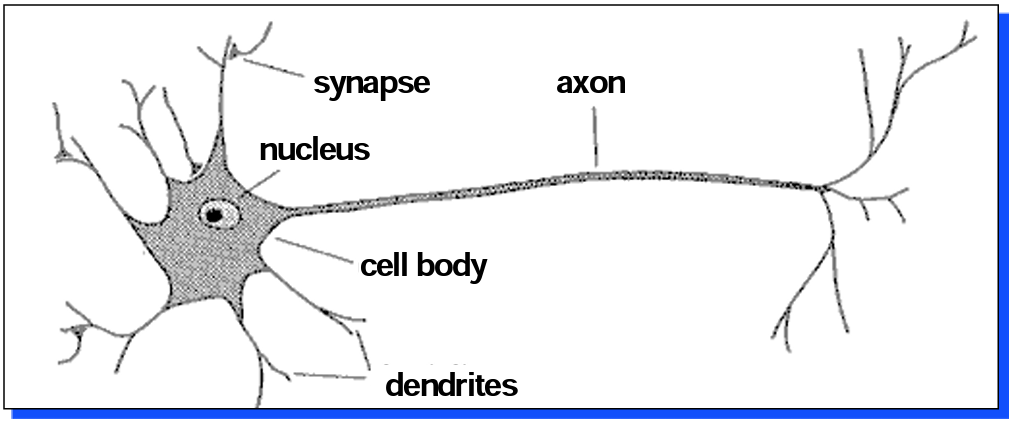
\includegraphics[width=0.5\linewidth]{tex/img/Structure_of_Neurons.PNG}
    \caption{The structure of Neurons}
    \label{fig:Neuron structure}
\end{figure}
A neuron has a cell body, a branching input structure (the dendrite), and a branching output structure (the axon). Axons connect to dendrites via synapses, Electro-chemical signals are propagated from the dendritic input, through the cell body, and down the axon to other neurons


\subsubsection{Perceptron}
A single neuron of a neural network is called a perceptron. A perceptron implements a mathematical function that operates on the input signals and generates outputs. Figure is an example of a perceptron. A perceptron is the simplest neural network.
\subsubsection{The learning process}
The perceptron model begins with the multiplication of all input values and their weights, then adds these values together to create the weighted sum. Then this weighted sum is applied to the activation function 'f' to obtain the desired output. This activation function is also known as the step function and is represented by 'f'. This step function or Activation function plays a vital role in ensuring that output is mapped between required values (0,1) or (-1,1). It is important to note that the weight of input is indicative of the strength of a node. Similarly, an input's bias value gives the ability to shift the activation function curve up or down.
The inputs to the neuron come either from the source (camera or sensing devices) or from the outputs of other neurons.

\begin{figure}[H]
    \centering
    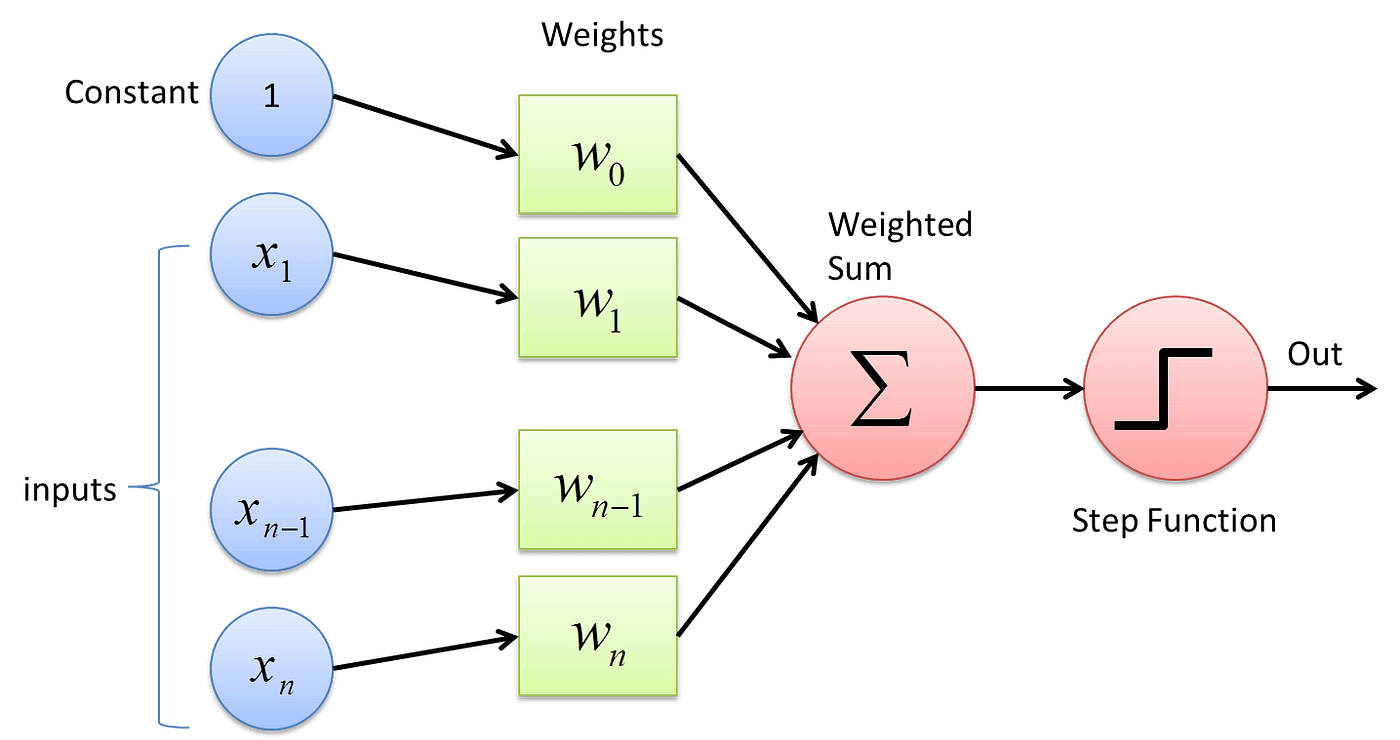
\includegraphics[width=0.7\linewidth]{tex/img/Perceptron.png}
    \caption{Perceptron}
    \label{fig:Perceptron}
\end{figure}

Mathematically, the output (y) of a neuron in a neural network perceptron can be expressed as:\\

\(y=f(\sum_{i=1}^{n}(\omega_{i}.x_{i})+b)\)

where:\\
$\omega_{i}$ is the weight associated with the input \(x_{i}\)\\
\(b\) is the bias term,\\
\(f:\) activation\\
As shown in fig \ref{fig:Perceptron}, One percepteron has the following components: \\
\begin{itemize}
    \item \textbf{Input Nodes or Input Layer: } The input layer, also known as the input nodes, is the first layer in a neural network. It is responsible for receiving the input data, which can be anything from numerical values to images or text. The input layer doesn't perform any computations or transformations on the input data, it merely passes it along to the subsequent layers in the network. \\
    \item \textbf{Weight: } Weights are parameters that adjust the strength of the connections between neurons (nodes) in adjacent layers of a neural network. Each connection has an associated weight, and these weights are learnable and updated during the training process. The weights determine the impact of the input signals on the neurons in the next layer. A higher weight means that the corresponding input has a stronger influence on the neuron's output. During training, the neural network adjusts these weights to minimize the difference between the predicted output and the actual target output. \\
    \item \textbf{Bias: } Biases are additional parameters in a neural network that allows for fine-tuning the output of each neuron. Unlike weights, biases are not associated with specific inputs but are added to the weighted sum of inputs in each neuron.
    Role: Biases provide the neural network with flexibility, enabling it to account for situations where all inputs are zero or have low values. They allow neurons to activate even when the weighted sum of inputs is not sufficient to trigger an output. Like weights, biases are adjusted during training to improve the network's overall performance. \\
    \item \textbf{Activation Function: } The primary purpose of an activation function is to determine whether a neuron should be activated (output a signal) or not, based on the input it receives.
    An activation function is a mathematical operation applied to the output of a neuron (or node) in a neural network. It introduces non-linearity to the network, allowing it to learn complex patterns and make more sophisticated decisions. The activation function takes the weighted sum of inputs and a bias term and produces the output of the neuron.\cite{nielsen2015neural}

\end{itemize}

\subsubsection{Types of Perceptron:}
Based on the layers, Perceptron models are divided into two types.
\begin{enumerate}
    \item \textbf{Single-layer Perceptron Model: } This is one of the easiest Artificial neural network (ANN) types. A single-layered perceptron model consists feed-forward network and also includes a threshold transfer function inside the model. The main objective of the single-layer perceptron model is to analyze the linearly separable objects with binary outcomes.

    In a single-layer perceptron model, its algorithms do not contain recorded data, so it begins with an inconstantly allocated input for weight parameters. Further, it sums up all inputs (weight). After adding all inputs, if the total sum of all inputs is more than a predetermined value, the model gets activated and shows the output value as +1.
    
    If the outcome is the same as the pre-determined threshold value, then the performance of this model is stated as satisfied, and weight demand does not change. However, this model consists of a few discrepancies triggered when multiple weight input values are fed into the model. Hence, to find the desired output and minimize errors, some changes should be necessary for the weights input.
    "Single-layer perceptron can learn only linearly separable patterns."\cite{ansari2020building}, \cite{knerr1990single}
    \item \textbf{Multi-layer Perceptron model: } Much like the human brain contains billions of neurons, an artificial neural network contains several neurons or perceptrons. Inputs are processed by a group of neurons. Each neuron in the group processes the inputs independently. Outputs from this group of neurons are fed to another neuron or group of neurons for further processing. You can imagine these neurons arranged as layers where the output from one layer is fed as inputs to the next layer. You can have as many layers as needed to train your neural network. This multilayer approach of arranging neurons in a neural network is commonly known as multilayer perceptron (MLP). Like a single-layer perceptron model, a multi-layer perceptron model also has the same model structure but has a greater number of hidden layers.
    \begin{figure}[H]
        \centering
        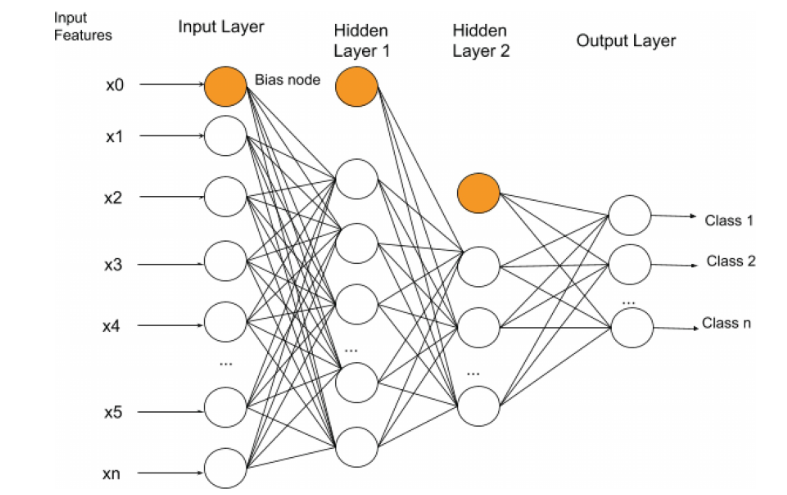
\includegraphics[width=0.8\linewidth]{tex/img/MLP.PNG}
        \caption{Multi layer perceptron}
        \label{fig:MLP}
    \end{figure}
    also known as the Backpropagation algorithm, which executes in two stages as follows:
    \begin{itemize}
        \item \textbf{Forward Stage:} Activation functions start from the input layer in the forward stage and terminate on the output layer.
        \item \textbf{Backward Stage:} In the backward stage, weight and bias values are modified as per the model's requirement. In this stage, the error between actual output and demand originated backward on the output layer and ended on the input layer.
    \end{itemize}
    A multi-layer perceptron model has greater processing power and can process linear and non-linear patterns. Further, it can also implement logic gates such as AND, OR, XOR, NAND, NOT, XNOR, and NOR.
    
    Hence, a multi-layered perceptron model is considered as multiple artificial neural networks having various layers in which the activation function does not remain linear, similar to a single-layer perceptron model. Instead of linear, the activation function can be executed as sigmoid, TanH, ReLU, etc., for deployment. \cite{ansari2020building}, \cite{nielsen2015neural}
\end{enumerate}

\subsection{Deep Learning}
Deep learning is another name for a multilayer artificial neural network or multilayer perceptron. Deep learning is the subset of machine learning methods that are based on artificial neural networks with representation learning. The adjective "deep" in deep learning refers to the use of multiple layers in the network. Methods used can be either supervised, semi-supervised, or unsupervised \cite{vargas2017deep}

Deep-learning architectures such as deep neural networks, deep belief networks, deep reinforcement learning, recurrent neural networks, convolutional neural networks, and transformers have been applied to fields including computer vision, speech recognition, natural language processing, machine translation, bioinformatics, drug design, medical image analysis, climate science, material inspection and board game programs, where they have produced results comparable to and in some cases surpassing human expert performance. \cite{hosseini2020deep}

\subsubsection{Deep Learning or Multilayer Perceptron Architecture}
A multilayer perceptron consists of at least three types of layers: input layer, hidden layers, and output layer. You can have more than one hidden layer. Each layer contains one or more neurons. A neuron performs some computation on the inputs it gets and generates outputs. The output from the neurons is sent as input to the next layer except in the case of the output layer,

\begin{enumerate}
    \item \textbf{Input layer: } This is the primary component of Perceptron which accepts the initial data into the system for further processing. Each input node contains a real numerical value.
    In a neural network, the input layer is the initial layer that receives the raw input data and passes it to the next layer in the network. Each node in the input layer represents a feature or an attribute of the input data. These nodes act as receptors for the raw input information and are connected to the nodes in the next layer, which is typically a hidden layer.
    
    Here are some key points about the input layer:
    \begin{enumerate}
        \item -Nodes/Neurons: The nodes in the input layer are also called input neurons. Each neuron corresponds to a specific feature or dimension of the input data.
        \item -Input Features: If you're working with a dataset of, for example, images, each node in the input layer might represent a pixel's intensity or color values. In the case of text data, each node could represent a unique word or a character.
        \item -No Processing: The nodes in the input layer do not perform any processing on the input data. They simply pass the raw input values to the next layer. The actual computation and learning occur in the subsequent layers, particularly in the hidden layers.
        \item -Connections: Each node in the input layer is connected to every node in the next layer (usually a hidden layer) through weights. These weights determine the strength of the connection between nodes and play a crucial role in the learning process of the neural network.
    \end{enumerate}
    The number of neurons in the input layer is the same as the number of features. Sometimes, an additional node is added in each layer. This additional node is called a bias node. The bias node is added to have control over the output from the layer. In deep learning, the bias is not required, but it is a common practice to add one.\\
    
    \textbf{Total Number of Neurons in the input layer} = The number of input features without a bias = (The number of input features + 1) with a bias 
    \cite{ansari2020building}\\
    \item \textbf{Hidden Layers: } Hidden layers are the layers in a neural network that come between the input layer and the output layer. These layers are called "hidden" because their outputs are not directly observable or part of the final network output during the training phase. A neural network must have at least one hidden layer. This is the layer where the learning happens. The neurons in this layer do the computations needed for learning. In most cases, one hidden layer is sufficient for learning, but you can have as many layers as needed to model the real-world cases. As the number of hidden layers increases, the computation complexity increases with a corresponding increase in computation time.
    \\
    
    \textbf{Total Number of Neurons in the hidden layer} = A common practice is to take two-thirds (or 66 percent) of the number of neurons in the previous layer.\\
    
    For example, if the number of neurons in the input layer is 100, the number of neurons in the first hidden layer will be 66 and in the next hidden layer will be 43, and so on. Again, there is no magic number, and you should tune the neuron counts based on the model accuracy.
    \item \textbf{Output Layer: } The output layer is the final layer in a neural network, responsible for producing the model's predictions or outputs based on the learned representations from the preceding layers. The number of neurons in the output layer depends on the type of problem you want the neural network to solve and is described here: \\
    \textbf{Nodes in the Output Layer can be used for:}
    \begin{itemize}
        \item \textbf{For binary classification: } there is typically one node with a sigmoid activation function, producing a probability output.\\
        \item \textbf{For multi-class classification: } when the network has to predict one of many classes, the output layer has as many neurons as the number of all possible classes.\\
        \item \textbf{For regression tasks: } there is usually a single node with a linear activation function, producing a continuous output/ when the network has to predict a continuous value, such as the closing price of stocks, the output node has only one neuron. \cite{calin2020deep}, \cite{nielsen2015neural}
    \end{itemize}
\end{enumerate}
\subsubsection{Forwardpropagation}

A feedforward neural network is an artificial neural network consisting of neurons with connections that do not form a cycle. This type of network is the simplest form of neural network and information flows in one direction, from the input layer to the hidden layer and then to the output layer. Unlike other types of neural networks, a feedforward neural network has no loopback or feedback mechanism. \cite{coates2011analysis} \cite{ansari2020building} \href{https://ml-cheatsheet.readthedocs.io/en/latest/forwardpropagation.html}{\textcolor{blue}{Source}}
\begin{figure}[H]
    \centering
    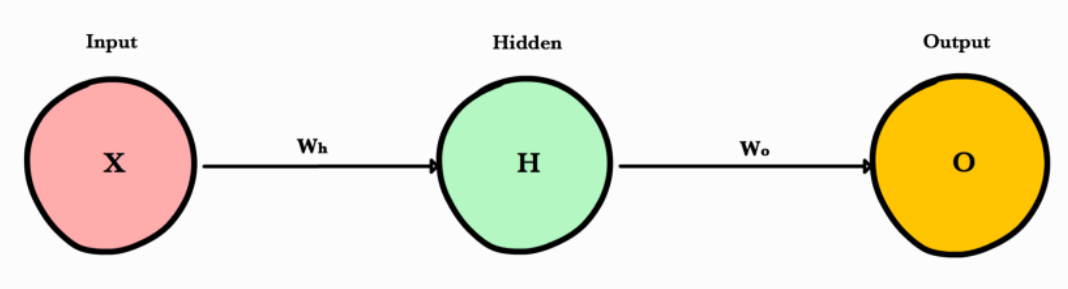
\includegraphics[width=0.7\linewidth]{tex/img/Forwardpropagation.PNG}
    \caption{Simple Network}
    \label{fig:enter-label}
\end{figure}
a single pass of forward propagation translates mathematically to:
\[Prediction=A(A(XW_{h})W_{o})\]
Where A:    is an activation function like ReLU, X is the input and $W_{h}$ and $W_{o}$ are weights.\\

\textbf{Steps}\\
- Calculate the weighted input to the hidden layer by multiplying X by the hidden weight $W_{h}$.\\
- Apply the activation function and pass the result to the final layer \\
- Repeat step 2 except this time X is replaced by the hidden layer’s output, H \cite{ansari2020building}, \cite{nielsen2015neural}

\subsubsection{BackPropagation: }
The goals of backpropagation are straightforward: adjust each weight in the network in proportion to how much it contributes to overall error. If we iteratively reduce each weight’s error, eventually we’ll have a series of weights that produce good predictions.\\
Here are the final 3 equations that together form the foundation of backpropagation. \cite{hecht1992theory} \cite{nielsen2015neural}
 \[
 Output Layer Error    E_{o} = (O-y).R'(Z_{o})
 \]
 \[ 
 Hidden Layer Error    E_{h} = E_{o}.W_{o}.R'(Z_{h})
 \]
 \[ 
 Cost-Weights Deriv \hspace{3mm}   LayerError.LayerInputs
 \]


\begin{figure}[H]
    \centering
    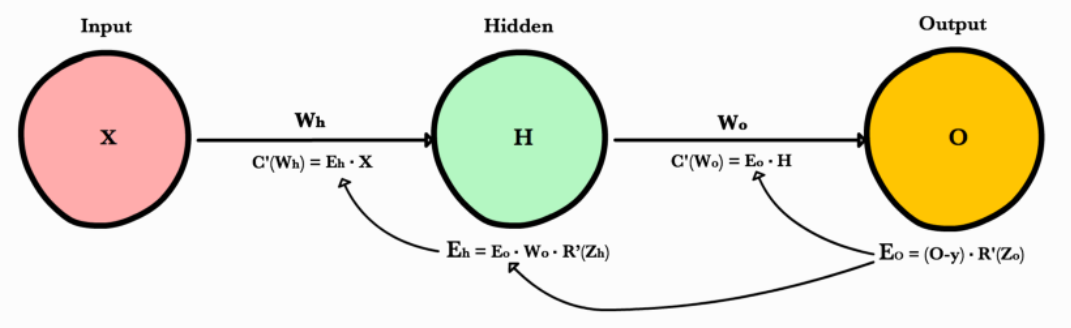
\includegraphics[width=0.8\linewidth]{tex/img/backward_propagation.PNG}
    \caption{Backward Propagation}
    \label{fig:backward_propagation}
\end{figure}
\subsubsection{Activation function}
The activation function determines whether the neuron it’s attached to should be activated (turned on or off), based on whether the neuron’s input is relevant for model prediction. The activation function normalized the output of each neuron to a range between 0 and 1 or between -1 and 1. Several mathematical functions are used as activation for different uses. \cite{sharma2017activation}, \cite{apicella2021survey}, \cite{bfortuner_mlglossary}

we can broadly divide the activation function into two: \\
\begin{itemize}
    \item \textbf{Linear Activation Function: } Commonly used in the output layer for regression tasks where a continuous range of values is desired. A linear activation function computes a weighted sum of its input without introducing non-linearity, and The output is a linear transformation of the input. 
    \begin{figure}[H]
        \centering
        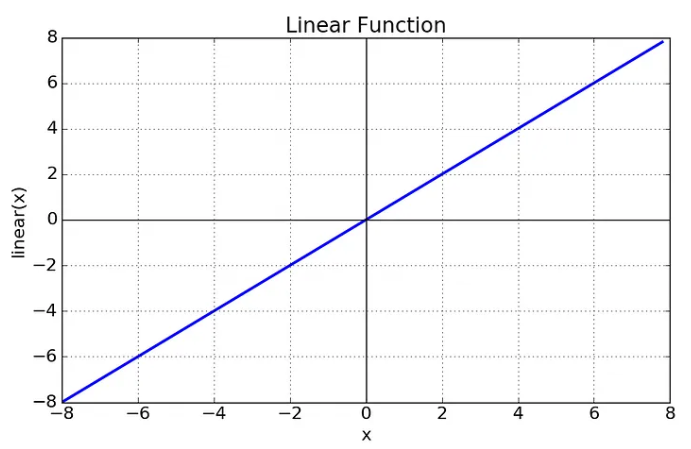
\includegraphics[width=0.5\linewidth]{tex/img/Linear_function.PNG}
        \caption{Linear Activation Function}
        \label{fig:LAF}
    \end{figure}
    \textbf{Equation: }
    \(f(x)=cx\) \\where c is constant.\\
    
    The output of the linear activation function varies from $-\infty$ to  $+\infty$, as shown in Figure above.
     If you choose to use a linear activation function, the last layer of your neural network will simply be a linear function of the first layer, regardless of how many layers the network has. This means that your network can only learn linear dependencies between the input and output, which is insufficient for solving complex problems like computer vision. Therefore, using a linear activation function is not recommended for such problems. \cite{bfortuner_mlglossary}\\
     \item \textbf{Non-linear Activation Function: } A non-linear activation function introduces non-linearity into the network, enabling it to learn complex relationships and representations. It facilitates the model's ability to generalize and differentiate outputs with diverse data.
    \begin{figure}[H]
        \centering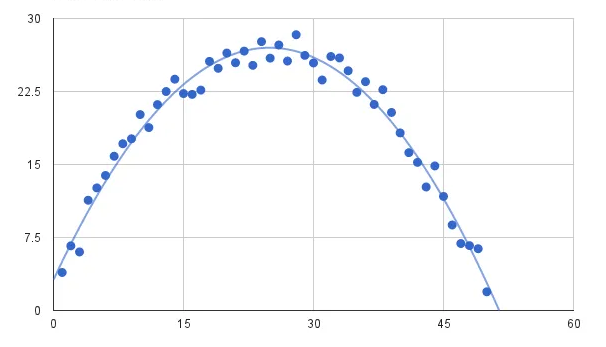
\includegraphics[width=0.5\textwidth]{Non-Linear.PNG}
        \caption{Non-Linear Activation Function}
    \end{figure}
    Essential for training deep neural networks as it allows the network to capture complex patterns and relationships in the data, They allow the network to capture intricate relationships between features, which is crucial for tasks like image recognition, natural language processing, and more.
    \begin{enumerate}
        \item \textbf{Sigmoid or Logistic Activation Function: } 
    The sigmoid activation function calculates the neuron output using the sigmoid function, as shown here:
    $$\phi(z)=\frac{1}{1+e^{-z}}$$
    \begin{figure}[H]
        \centering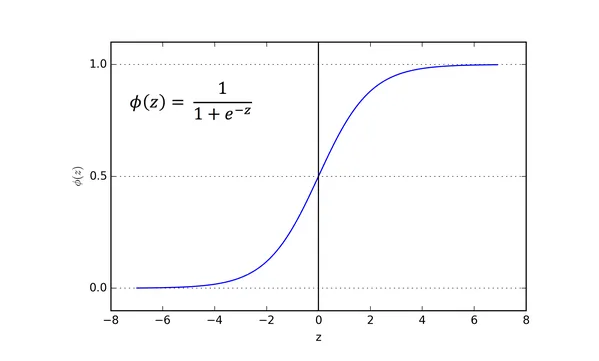
\includegraphics[width=0.5\textwidth]{sigmoid_Activation.PNG}
        \caption{Sigmoid Activation Functioin}
    \end{figure}
    where \(z\) is calculated like \\
    
    $$z=X_0+\sum_{i=0}^{i=n}w_{i}x_{i}$$
    
    The sigmoid function always yields a value between 0 and 1. This makes the output smooth without many jumps as the input value fluctuates. The other advantage is that this is a nonlinear function and does not generate a constant value from a first-order derivative.
    
    The sigmoid function is a mathematical function that always produces an output value between 0 and 1. This characteristic results in a smooth output without many jumps as the input value fluctuates. Another benefit of the sigmoid function is that it is nonlinear, and its first-order derivative does not generate a constant value.
    \item \textbf{Tanh or hyperbolic tangent Activation Function}
    
    TanH is similar to the sigmoid activation function except that TanH is zero-centered and The range of the tanh function is from (-1 to 1).
    
    \begin{figure}[H]
        \centering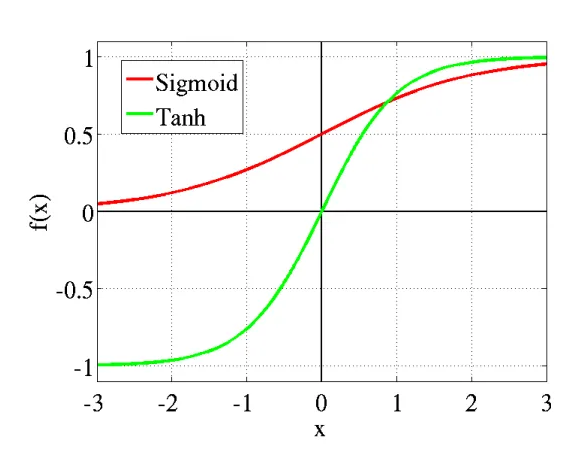
\includegraphics[width=0.5\textwidth]{Tangent_activation.PNG}
        \caption{Tangent Activation Functioin}
    \end{figure}
    
    The TanH activation function calculates the neuron output using:\\
    $$tanh(z)=\frac{e^{z}-e^{-z}}{e^{z}+e^{-z}}$$
    The advantage is that the negative inputs will be mapped strongly negative and the zero inputs will be mapped near zero in the tanh graph.
    \item \textbf{ReLU (Rectified Linear Unit) Activation Function)}
    ReLU is widely used for most computer vision model training as the image pixels do not have negative values. The advantage of the ReLU activation function is that it is computationally efficient and allows the network to converge quickly. Also, ReLU is nonlinear, and it has a derivative function that makes it suitable for backpropagation for weight adjustment as the neural network learns.
    
    \begin{figure}[H]
        \centering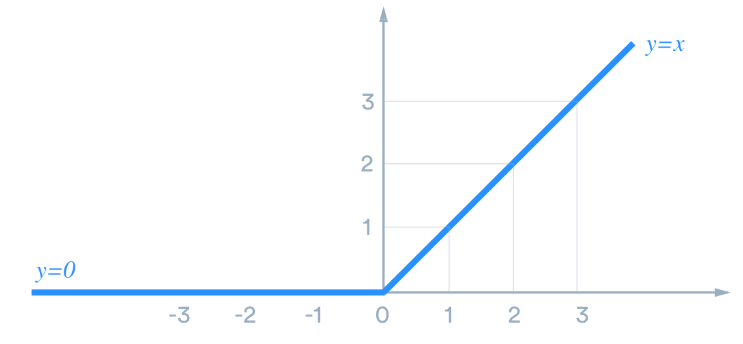
\includegraphics[width=0.5\textwidth]{Relu_Activation.PNG}
        \caption{ReLU Activation Functioin}
    \end{figure}
    
    ReLU is widely used for most computer vision model training as the image pixels do not have negative values.
    
    $$f(x)=max(0,x)$$
    it ranges from 0 to +$\infty$\\
    \item  \textbf{Leaky ReLU Activation Function}
    The leaky ReLU has a small slope in the negative area and allows for backpropagation for negative inputs.
    
    The disadvantage is that the result of the leaky ReLU is not consistent with negative values.
    \begin{figure}[H]
        \centering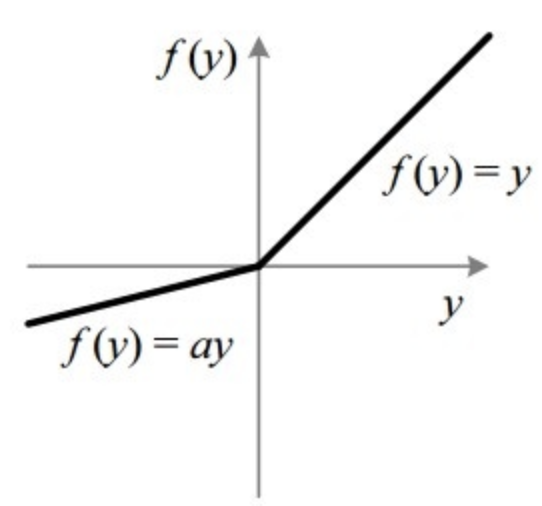
\includegraphics[width=0.5\textwidth]{leaky_relu.png}
        \caption{Leaky ReLU Activation Functioin}
    \end{figure}
    
    $f(y)=\left\{\begin{array}{rcl}
         \alpha y & \mbox{for} & y<0\\
         y & \mbox{for} & y\geq 0
    \end{array}\right.$\\
    \item \textbf{SELU Actiovation Function}
    A scaled exponential linear unit (SELU) computes neuron outputs using the following equation:
    
    $f(\alpha,x)=\lambda\left\{\begin{array}{rcl}
         \alpha (e^{x}-1) & \mbox{for} & x<0\\
          x & \mbox{for} & x\geq 0
    \end{array}\right.$\\
    \\
    where the value of $\lambda$ = 1.05070098 and the value of $\alpha$ = 1.67326324. These values are fixed and do not change during backpropagation.[Orielly]
    \begin{figure}[H]
        \centering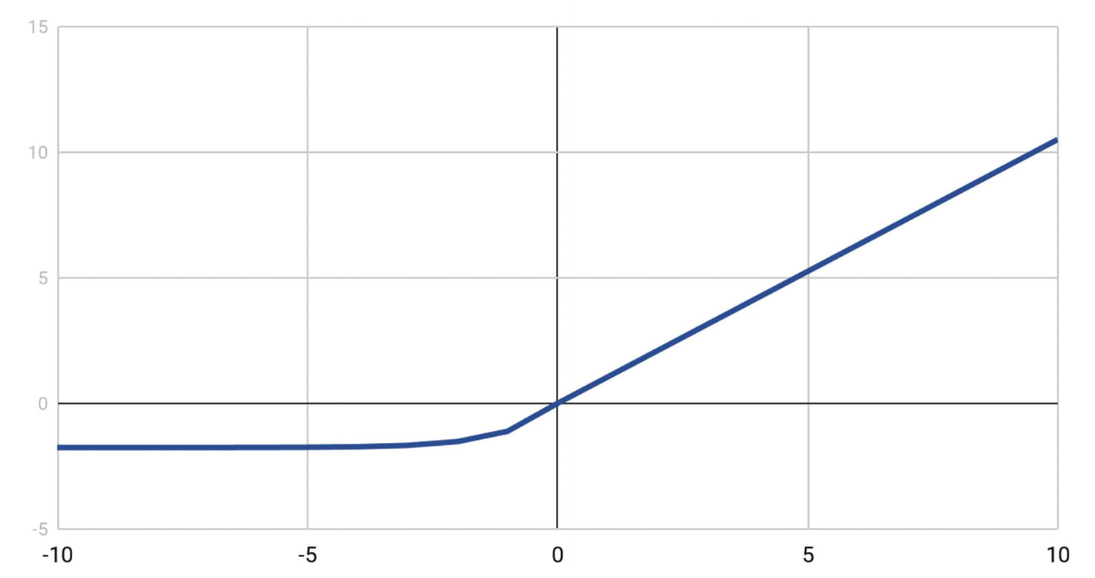
\includegraphics[width=0.5\textwidth]{SELU_activation.PNG}
        \caption{SELU Activation Functioin}
    \end{figure}
    
    SELU has the “self-normalizing” properties, Since with SELU the entire network is self-normalizing, it is efficient in terms of computation and tends to converge faster. Another advantage is that it overcomes the problems of exploding or vanishing gradients when the input features are too high or too low.
    \item \textbf{Softplus Activation Function}
    The softplus activation function applies smoothing to the activation function value 
    \(z\) . It uses the log of exponent as follows:\\
    
    $$f(x)=ln(1+e^{z})$$\\
    \\
    Softplus is also called the SmoothReLU function. The first derivation of the softplus function is  $\frac{1}{1+e^{z}}$, which is the same as the sigmoid activation function. 
    
    \begin{figure}[H]
        \centering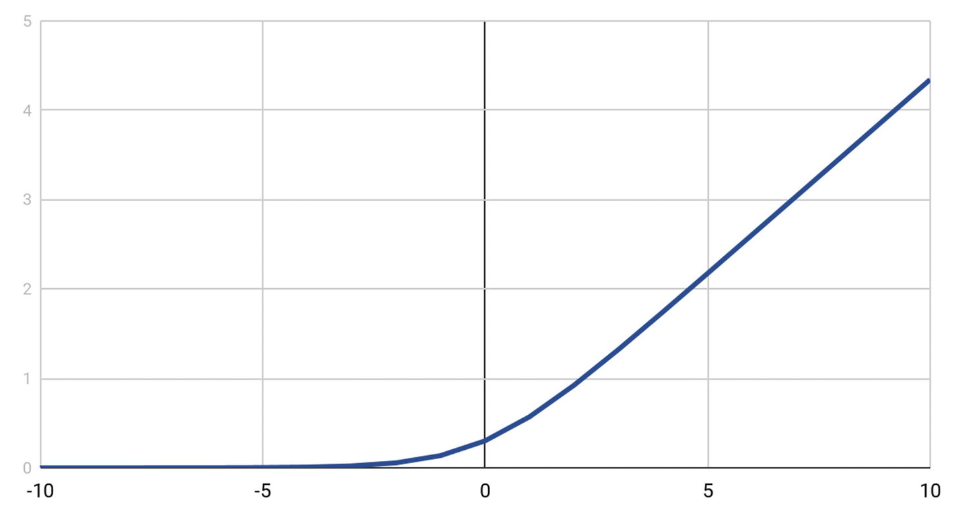
\includegraphics[width=0.5\textwidth]{Softplus_activation.PNG}
        \caption{Softplus Activation Function}
    \end{figure}
    \item \textbf{Softmax}
    The Softmax function takes a vector of real numbers as input, normalizes it to create a probability distribution, and generates outputs between the values 0 and 1 such that the sum of all output values is equal to 1. 
    
    This function is most commonly used as the activation function for the output layer of a classification neural network. The resulting output values are interpreted as prediction probabilities for each class.
    \begin{figure}[H]
        \centering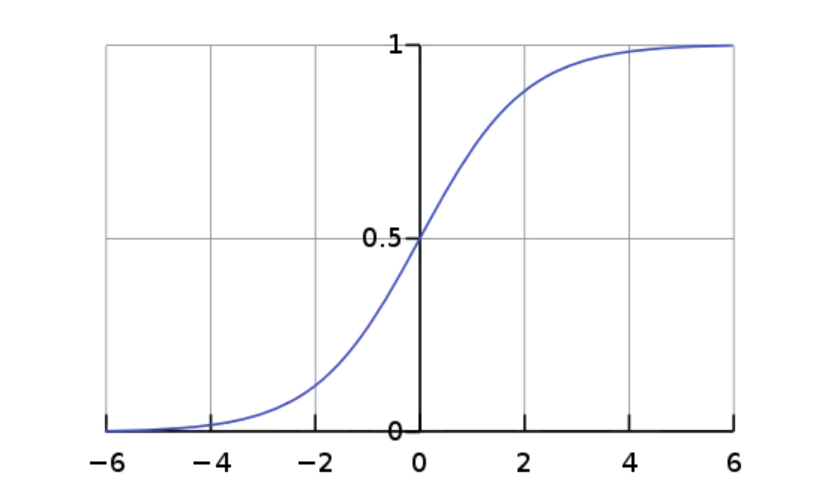
\includegraphics[width=0.5\textwidth]{Softmax.PNG}
        \caption{Softmax Activation Function}
    \end{figure}
    $$\sigma(z)_{i}=\frac{e^{z_{i}}}{\sum_{j=1}^{k}e^{z_{j}}}$$ for \(i\)=1,...., k and z=$(z_{1}....,z_{k})$ $\epsilon R^{k}$
    \end{enumerate}
\end{itemize}

\subsubsection{Loss Function/Error Function}
A loss function is a function that compares the target and predicted output values; and measures how well the neural network models the training data. When training, we aim to minimize this loss between the predicted and target outputs.
The equation of error may be written in a simplified form as follows:\\

\(Error = Expected outcome - Predicted outcome\)\\

When a neural network begins the learning process, it initializes weights and calculates output from each neuron using an activation function. It then computes the error, adjusts the weights, recalculates outputs, and re-evaluates errors, until it reaches the minimum error. The weights that give the minimum errors are considered the final weights and the network is considered "learned" at this stage.

In calculus, if the first derivative of a function is zero, then the function at that point is either a minimum or a maximum. The neural network training process aims to find the minimum point where the first derivative is zero. To achieve this, a neural network must have an \textbf{error function} that calculates the first derivative and identifies the points (weights and biases) where the error function is minimum. The type of error function used depends on the type of model being trained. These error functions are also called loss functions or simply losses.\\

The error functions are broadly divided into the following three categories: \cite{ansari2020building}, \cite{heaton2018ian}\\
\begin{itemize}
    \item \textbf{Regression loss functions} are used when we want to train models to predict continuous value outcomes, typically a numerical value. To measure the difference between the predicted and actual target values, different loss functions are employed. The following are some widely used regression loss functions:\\
    \begin{itemize}
    \item \textbf{Mean Squared Error (MSE) Loss:} This is the default error function for regression problems. This is the preferred loss function if the distribution of the target variable is normal or Gaussian. This function has numerous properties that make it especially suited for calculating loss. The difference is squared, which means it does not matter whether the predicted value is above or below the target value; however, values with a large error are penalized.\\
    $$MSE=\frac{1}{n}\sum_{i=1}^{n}(y^{(i)}-\hat{y}^{(i)})^{2}$$
    \item  \textbf{Mean Absolute Error (MAE) Loss:}  MAE finds the average of the absolute differences between the target and the predicted outputs.
    $$MAE=\frac{1}{n}\sum_{i=1}^{n}|y^{(i)}-\hat{y}^{(i)}|$$
    In some cases, this loss function serves as an alternative to MSE. As mentioned earlier, MSE is highly sensitive to outliers, which can significantly affect the loss due to the squared distance. To mitigate this, MAE is used when the training data has a substantial number of outliers.
    \item \textbf{The Mean Squared Logarithmic Error (MSLE) is a loss function}  used in regression tasks, particularly when the target values span several orders of magnitude. MSLE measures the mean squared difference between the natural logarithm of the predicted values and the natural logarithm of the true values. This can be especially useful when the scale of the target values varies widely.
    The formula for MSLE is as follows:
     $$MSLE(y,\hat{y})=\frac{1}{n}\sum_{i=1}^{n}(log(1+y^{(i))}-log(1+\hat{y}^{(i)}))^{2}$$
     where: \\
     $y^{i}: $ is the true target value for the \(i\)-th sample.\\
     $\hat{y}^{(i)}: $ is the predicted target value for the \(i\)-th sample.
     \item \textbf{Huber Loss: } The Huber loss, also referred to as the smooth L1 loss, is a commonly used loss function in regression tasks. It is designed to be less sensitive to outliers compared to the Mean Squared Error (MSE) loss function while retaining the benefits of a quadratic loss function for smaller errors.

     $$Huber(y,\hat{y})=\frac{1}{n}\sum_{i=1}^{n}L_{\delta}(y^{(i))}-\hat{y}^{(i)})$$
     where: \\
     $y_{i}: $ is the true target value for the \(i\)-th sample.\\
      $y^{i}: $ is the predicted target value for the \(i\)-th sample.\\
      $n: $ is the total number of samples.\\
      $L_{\delta}(x)$ is defined as:
      
      $L_{\delta}(x)=\left\{\begin{array}{rcl}
           \frac{1}{2}x^{2} & \mbox{for} & |x| \leq \delta \\
          \delta(|x|-\frac{1}{2}\delta) & otherwise 
      \end{array}\right.$\\
      \textbf{Benefit: } One big When training neural networks, using Mean Absolute Error (MAE) can cause a problem due to its large gradient, which can result in missing the minima at the end of training when using gradient descent. In contrast, as the loss gets closer to its minima, the gradient decreases when using Mean Squared Error (MSE), making it more accurate.
    
    To address this issue, Huber loss can be very useful since it curves around the minima, decreasing the gradient. Additionally, Huber loss is more resistant to outliers than MSE. Therefore, it combines the desirable properties of both MSE and MAE.
    \item  \textbf{Log-Cosh loss: } The Log-Cosh loss is a smooth and differentiable approximation of the Huber loss, often used in regression tasks. Similar to the Huber loss, it aims to be less sensitive to outliers than the Mean Squared Error (MSE) loss, but it has the advantage of being continuously differentiable.
     $$Log-Cosh(y,\hat{y})=\frac{1}{n}\sum_{i=1}^{n}Log(cosh(y^{(i))}-\hat{y}^{(i)}))$$
     where: \\
      $y_{i}: $ is the true target value for the \(i\)-th sample.\\
      $y^{i}: $ is the predicted target value for the \(i\)-th sample.\\
      $n: $ is the total number of samples.\\
      \(Cosh: \) is the hyperbolic cosine function.\\
      The optimization goal during training is to minimize the Log-Cosh loss, and the model adjusts its parameters to achieve predictions that result in smaller Log-Cosh loss values. The Log-Cosh loss is often considered when a balance between the robustness of the Huber loss and the differentiability of the MSE loss is desired.
      \item \textbf{Quantile loss function: } Quantile loss is a loss function used in quantile regression, where the goal is to predict not just a central tendency (like the mean in traditional regression) but rather different quantiles of the target distribution. It is particularly useful when you want to estimate a range of possible values for a prediction.
      $$L_{\gamma}(y, y^{p})=\sum_{i=y_{i}<y_{i}^{p}}(\gamma-1).|y_{i}-{y_{i}^{p}}|+ \sum_{i=y_{i}\geq y_{i}^{p}}(\gamma).|y_{i}-y_{i}^{p}|$$

      The optimization goal during training is to minimize the Quantile Loss, and the model adjusts its parameters to achieve predictions that capture the desired quantiles of the target distribution. Quantile regression is particularly useful in scenarios where understanding the variability or uncertainty in predictions is essential.
      
    
     
    \end{itemize}
    \item \textbf{Binary classification loss functions} are used when we want to train models to predict a maximum of two classes (usually denoted as 0 and 1) and the true binary label, such as cat versus dog or cancer versus no cancer. \\
          \begin{itemize}
          \item \textbf{Binary Crossentropy Loss (Log Loss): } This is the default loss function for binary classification problems and is preferred over other functions. Cross-entropy calculates a score that summarizes the average difference between the actual and predicted probability distributions for predicting class 1. The score is minimized, and a perfect cross-entropy value is set to 0.  
          and can be used When the target value is in the range (0,1).
          $$Binary Crossentropy(y, \hat{y})=\frac{1}{n}\sum_{i=1}^{n}[y_{i}log(\hat{y_{i}})+(1-y_{i})log(1-\hat{y_{i}})]$$

          It measures the cross-entropy between the true binary labels and the predicted probabilities. It penalizes deviations from the true labels by assigning higher penalties to confidently wrong predictions.
          \item \textbf{Hinge Loss (SVM Loss):} This is used mainly in support of vector machine–based binary classification and can be used when the target variable is in the range (-1, 1).
          $$Hinge-Loss(y,\hat{y})= \frac{1}{n}\sum_{i=1}^{n}max(0,1-y_{i}.\hat{y_{i}})$$

          Penalizes misclassifications linearly and encourages correct predictions to have a margin of at least 1.

          \item \textbf{Squared Hinge Loss: } This function calculates the square of the score hinge loss. It smoothens the surface of the error function and makes it numerically easier to work with.
          \[
          \text{Squared Hinge Loss}(y,\hat{y})=\frac{1}{n}\sum_{i=1}^{n}max(0,1-y_{i}.\hat{y_{i}})^{2}
          \]
      \end{itemize}
    \item \textbf{Multiclass classification loss functions} are used when our models need to predict more than two classes/are used to measure the difference between predicted class probabilities and true class labels in scenarios where there are more than two classes, such as object detection. \\
          \begin{itemize}
          \item \textbf{Categorical Crossentropy Loss: } used for multiclass classification tasks with one-hot encoded true class labels. It measures the cross entropy between the true distribution and the predicted class probabilities.
          $$Categorical Crossentropy(y,\hat{y_{i}})=-\frac{1}{n}\sum_{i=1}^{n}\sum_{j=1}^{m}y_{ij}log(\hat{y_{ij}})$$
          \item \textbf{Sparse Categorical Crossentropy Loss: } Similar to Categorical Crossentropy but used when the true class labels are provided as integers rather than one-hot encoded vectors.
          $$Sparse Categorical Crossentropy(y,\hat{y})=-\frac{1}{n}\sum_{i=1}^{n}log(\hat{y_{i}[y_{i}]})$$
          Sparse cross-entropy performs the same cross-entropy calculation of error without requiring that the target variable be one hot-encoded before training and is used When you have a large number of classes in the target, for example, predicting dictionary words.
          \item \textbf{Kullback-Leibler divergence (KLD) loss: } KLD measures how one probability distribution differs from a baseline distribution. A KL divergence loss of 0 means the distributions are identical. It determines how much information is lost (in terms of bits) if the predicted probability distribution is used to approximate the desired target probability distribution.

        This is used to solve complex problems such as auto-encoders for learning dense features. If this is used for multiclass classification, it works as multiclass cross-entropy.
        \[
        \text{KL Divergence}(P \parallel Q) = \sum_{i \in \chi} P(i) \log\left(\frac{P(i)}{Q(i)}\right)
        \]
        where:\\
        For discrete probability distributions, P and Q are defined on the same sample space, $\chi$, the relative entropy from Q to P.
        \item \textbf{Cross-Entropy Loss (Sigmoid Crossentropy for Multilabel Classification): }
        Suitable for multilabel classification where each sample can belong to multiple classes. It measures the crossentropy for each class independently.

         \[
         \text{Cross Entropy Loss}(y,\hat{y})=-\frac{1}{n}\sum_{i=1}^{n}[y_{i}log(\sigma(\hat{y_{i}}))+(1-y_{i})log(1-\sigma(\hat{y_{i}}))]
         \]
      \end{itemize}

\end{itemize}

\subsubsection{Layers}
In a neural network, layers are the building blocks that organize and structure the computation. Each layer contains a group of nodes, or neurons, that process information.
\begin{itemize}
    \item \textbf{Convolutional Layer: } In CNN, convolution is a linear operation that involves the multiplication of weight (kernel/filter) with the input and it does most of the heavy lifting job. The convolution layer consists of 2 major components: \\
    \begin{itemize}
        \item \textbf{Kernel (Filter): } A convolution layer can have more than one filter. The size of the filter should be smaller than the size of the input dimension. It is intentional as it allows the filter to be applied multiple times at different points (positions) on the input. Filters are helpful in understanding and identifying important features from a given input. Applying different filters (more than one filter) on the same input helps in extracting different features from the given input. Output from multiplying the filter with the input gives a dimensional array. As such, the output array from this operation is called “Feature Map”.
        \item \textbf{Stride: } This property controls the movement of the filter over input. when the value is set to 1, then the filter moves 1 column at a time over input. When the value is set to 2 then the filer jumps 2 columns at a time as the filter moves over the input.
    \end{itemize}
    \item \textbf{Dropout Layer: } A dropout layer takes the output of the previous layer’s activations and randomly sets a certain fraction (dropout rate) of the activations to 0, canceling or ‘dropping’ them out.

    It is a common regularization technique used to prevent overfitting in Neural Networks.
    The dropout rate is the tunable hyperparameter that is adjusted to measure performance with different values. It is typically set between 0.2 and 0.5 (but maybe arbitrarily set).
    
    Dropout is only used during training; At test time, no activations are dropped, but scaled down by a factor of dropout rate. This is to account for more units being active during test time than training time. The premise behind dropout is to introduce noise into a layer to disrupt any interdependent learning or coincidental patterns that may occur between units in the layer, that aren’t significant. \\
    \item \textbf{Pooling layer: }Pooling layers often take convolution layers as input. A complicated dataset with many objects will require a large number of filters, each responsible for finding patterns in an image so the dimensionally of a convolutional layer can get large. It will cause an increase in parameters, which can lead to over-fitting. Pooling layers are methods for reducing this high dimensionally. Just like the convolution layer, there is kernel size and stride. The size of the kernel is smaller than the feature map. For most of the cases, the size of the kernel will be 2X2 and the stride of 2. There are mainly two types of pooling layers.

    The first type is the max pooling layer. The Max pooling layer will take a stack of feature maps (convolution layer) as input. The value of the node in the \textbf{max pooling layer} is calculated by just the maximum of the pixels contained in the window.
    
    The other type of pooling layer is the: \\
    \textbf{Average Pooling layer}. The average pooling layer calculates the average of pixels contained in the window. It's not used often but you may see this used in applications for which smoothing an image is preferable.\\
    \item \textbf{Fully-connected/Linear Layer: } In a neural network, a fully-connected layer, also known as a linear layer, is a type of layer where all the inputs from one layer are connected to every activation unit of the next layer. In most popular machine learning models, the last few layers in the network are fully-connected ones. Indeed, this type of layer performs the task of outputting a class prediction, based on the features learned in the previous layers.
    The fully-connected layer receives in input a vector of nodes, activated in the previous convolutional layers. This vector passes through one or more dense layers, before being sent to the output layer. Before it reaches the output layer, an activation function is used for making a prediction. While the convolutional and pooling layers generally use a ReLU function, the fully-connected layer can use two types of activation functions, based on the type of the classification problem:
    
    Sigmoid: A logistic function, used for binary classification problems.
    Softmax: A more generalized logistic activation function, it ensures that the values in the output layer sum up to 1. Commonly used for multi-class classification.
    The activation function outputs a vector whose dimension is equal to the number of classes to be predicted. The output vector yields a probability from 1 to 0 for each class. \cite{schmidhuber2015deep}, \cite{goodfellow2016deep}\\
   
\subsubsection{Optimizer}
An optimizer is an algorithm or method used to adjust the parameters of the neural network (weights and biases) during the training process. The primary goal of an optimizer is to minimize the loss function, which measures the difference between the predicted output and the true target values.

During training, the neural network makes predictions, and the optimizer adjusts the model's parameters based on the error (loss) between these predictions and the actual target values. The optimization process involves finding the optimal set of parameters that minimize the loss, enabling the neural network to make accurate predictions on unseen data. \cite{choi2019empirical}, \cite{ansari2020building} 

Some commonly used optimizers in neural networks include:
\begin{itemize}
    \item \textbf{Adaptive gradient (Adagrad): } adaptively sets the learning rate according to a parameter.
\begin{itemize}
    \item Parameters that have higher gradients or frequent updates should have slower learning rate so that we do not overshoot the minimum value.
    \item Parameters that have low gradients or infrequent updates should faster learning rate so that they get trained quickly.
    \item  It divides the learning rate by the sum of squares of all previous gradients of the parameter.
    \item When the sum of the squared past gradients has a high value, it basically divides the learning rate by a high value, so the learning rate will become less.
    \item Similarly, if the sum of the squared past gradients has a low value, it divides the learning rate by a lower value, so the learning rate value will become high.
    \item This implies that the learning rate is inversely proportional to the sum of the squares of all the previous gradients of the parameter.
    \end{itemize}
    \[
    g_{t}^{i}=\frac{\partial J(w_{t}^{i})}{\partial \mathbf{W}}
    \]
    \[
    \mathbf{W}=\mathbf{W}-\alpha\frac{\partial J(\omega_{t}^{t})}{\sqrt{\sum_{r=1}^{t}(g_{r}^{i})^2+\epsilon}}
    \]
    where: \\
     $g_{t}^{i}$  the gradient of a parameter\\
    $\alpha$ : the learning rate\\
    $\epsilon: $ very small value to avoid dividing by zero
    
    \item \textbf{Adaptive delta(Adadelta): }AdaDelta belongs to the family of stochastic gradient descent algorithms, that provide adaptive techniques for hyperparameter tuning. Adadelta is probably short for ‘adaptive delta’, where delta here refers to the difference between the current weight and the newly updated weight.
    Adadelta is a more robust extension of Adagrad that adapts learning rates based on a moving window of gradient updates, instead of accumulating all past gradients. This way, Adadelta continues learning even when many updates have been done.
    
    With Adadelta, we do not even need to set a default learning rate, as it has been eliminated from the update rule.
    
    \[
    v_{t}=\rho v_{t-1}+(1-\rho)\bigtriangledown_{\theta}^{2}J(\theta)
    \]
    \[
    \bigtriangleup\theta=\frac{\sqrt{\omega_{t}+\epsilon}}{\sqrt{v_{t}+\epsilon}}\bigtriangledown_{\theta}J(\theta)
    \]
    \[
    \theta=\theta-\eta\bigtriangleup\theta
    \]
    $\omega_{t}=\rho\omega_{t-1} + (1-\rho)\bigtriangleup\theta^{2}$
    \item \textbf{Adam Optimizer: } Adaptive Moment Estimation (Adam) combines ideas from both RMSProp and Momentum. It computes adaptive learning rates for each parameter and works as follows.
    \begin{itemize}
        \item First, it computes the exponentially weighted average of past gradients $(v_{dW})$
        \item Second, it computes the exponentially weighted average of the squares of past gradients $(s_{dW})$
        \item Third, these averages have a bias towards zero and to counteract this a bias correction is applied $(v_{dW}^{corrected}, s_{dW}^{corrected})$
        \item Lastly, the parameters are updated using the information from the calculated averages\\
        \[v_{dW}=\beta_{1}v_{dW}+(1-\beta_{1})\frac{\partial J}{\partial W}\]
        \[
        s_{dW}=\beta_{2}s_{dW}+(1-\beta_{2}) \left(\frac{\partial J}{\partial W}\right)^{2}
        \]
        \[
         v_{dW}^{corrected}=\frac{v_{dW}}{1-(\beta_{1})^{t}}
        \]
        \[
         s_{dW}^{corrected}=\frac{s_{dW}}{1-(\beta_{1})^{t}}
        \]
        \[
        W=W-\alpha\frac{v_{dW}^{corrected}}{\sqrt{s_{dW}^{corrected}} + \epsilon}
        \]
        where:\\
        $v_{dW}$-  the exponentially weighted average of past gradients\\
        $s_{dW}$- the exponentially weighted average of past squares of gradients\\
        $\beta_{1}$- hyperparameter to be tuned\\
        $\beta_{2}$- hyperparameter to be tuned\\
        $\frac{\partial J}{\partial W}$ - cost gradient with respect to current layer\\
        W- the weight matrix (parameter to be updated)\\
        $\alpha$ - the learning rate\\
        $\epsilon$ - very small value to avoid dividing by zero\\
    \end{itemize}
    \item \textbf{RMSProp Optimizer: } Another adaptive learning rate optimization algorithm, Root Mean Square Prop (RMSProp) works by keeping an exponentially weighted average of the squares of past gradients. RMSProp then divides the learning rate by this average to speed up convergence.
    \[
    s_{dW} = \beta s_{dW} + (1-\beta)\left(\frac{\partial J}{\partial W}\right)^{2}
    \]
    \[
    W = W-\alpha\frac{\frac{\partial J}{\partial W}}{\sqrt{s_{dW}^{corrected}}+ \epsilon}
    \]
    
    where: \\
    s - the exponentially weighted average of past squares of gradients\\
    $\frac{\partial J}{\partial W}$-  cost gradient with respect to current layer weight tensor\\
    W - weight tensor\\
    $\beta$- hyperparameter to be tuned\\
    $\alpha$- the learning rate\\
    $\epsilon$- very small value to avoid dividing by zero.
    \item \textbf{Stochastic Gradient Descent(SGD) Optimizer: } Stochastic Gradient Descent (SGD) is a widely used optimization algorithm for training neural networks and other machine learning models. It is a variant of the gradient descent optimization algorithm that processes each training example individually, rather than using the entire dataset in each iteration. This property makes it well-suited for large datasets. Optionally, partition the dataset into mini-batches of a fixed size.
    \begin{itemize}
        \item For each mini-batch or individual example:
        \item Compute the gradient of the loss with respect to the model parameters.
        \item Update the model parameters in the opposite direction of the gradient to minimize the loss.
    \end{itemize}.\\
    The update rule for the model parameters $\theta$ is given by:
    \[
    \theta_{t} = \theta_{t-1}-\alpha\bigtriangledown J(\theta_{t-1},x_{i}, y_{i})
    \]\\
    where: \\
    $\alpha : $  is the learning rate, a hyperparameter that controls the size of the steps taken during optimization.\\
    $\bigtriangledown J(\theta_{t-1},x_{i}, y_{i}$ is the gradient of the loss function $\mathbf{J}$ with respect to the parameters $\theta$ for the example $x_{i}, y_{i}$
\end{itemize}



\subsubsection{Regularization}
It is a Techniques for combating overfitting and improving training. Regularization methods introduce additional constraints or penalties to the training process, encouraging the model to be simpler and generalize better to unseen data. \cite{goodfellow2016deep}, \cite{ansari2020building}, \cite{bishop2006pattern}
\begin{itemize}
    \item \textbf{Data Augmentation: } \href{https://research.aimultiple.com/data-augmentation-techniques/}{\textcolor{blue}{Source}}
    Having more data is the surest way to get better consistent estimators (ML model), in contrast having a small dataset will lead to the well-known problem of overfitting.
    Data augmentation refers to the technique of artificially increasing the size of a dataset by applying various transformations to the existing data. This is often used in deep learning, particularly in computer vision tasks, to improve the performance of neural networks.
    There are various types of data augmentation techniques, including:
    \begin{enumerate}
        \item  Flipping: horizontally or vertically flipping an image.
        \item rotation: rotating an image by a certain degree.
        \item Zooming: zooming in or out of an image.
        \item Translation: shifting an image horizontally or vertically.
        \item Cropping: cropping a portion of an image.
        \item Adding noise: adding random noise to an image.
        
    \end{enumerate}
    
    These techniques can be used individually or in combination to generate new data samples. By increasing the size of the dataset, the neural network is exposed to more variations of the same data, which helps improve its ability to generalize and make accurate predictions on new, unseen data. \cite{shorten2019survey}\\
    \item \textbf{Dropout: } Dropout is a regularization technique for reducing overfitting in neural networks by preventing complex co-adaptations on training data.

    Dropout is a technique where randomly selected neurons are ignored during training. They are “dropped-out” randomly. This means that their contribution to the activation of downstream neurons is temporally removed on the forward pass and any weight updates are not applied to the neuron on the backward pass.
    
    Simply put, it is the process of ignoring some of the neurons in particular forward or backward pass.
    
    Dropout can be easily implemented by randomly selecting nodes to be dropped out with a given probability (e.g .1\%) each weight update cycle.
    
    Most importantly Dropout is only used during the training of a model and is not used when evaluating the model. \\
    \item \textbf{Early Stopping: } One alternative technique to prevent overfitting is use validation error to decide when to stop. This approach is called Early Stopping.
    One of the biggest problem in training neural network is how long to train the model.
    
    Training too little will lead to underfit in train and test sets. Traning too much will have the overfit in training set and poor result in test sets.
    
    Here the challenge is to train the network long enough that it is capable of learning the mapping from inputs to outputs, but not training the model so long that it overfits the training data.
    
    One possible solution to solve this problem is to treat the number of training epochs as a hyperparameter and train the model multiple times with different values, then select the number of epochs that result in the best accuracy on the train or a holdout test dataset, But the problem is it requires multiple models to be trained and discarded. \cite{goodfellow2016deep}\\
    \item \textbf{Ensembling: } Ensemble methods combine several machine learning techniques into one predictive model. There are a few different methods for ensembling, but the two most common are:
    \begin{itemize}
        \item \textbf{Bagging}Bagging stands for bootstrap aggregation. One way to reduce the variance of an estimate is to average together multiple estimates.
        It trains a large number of “strong” learners in parallel.
        A strong learner is a model that’s relatively unconstrained.
        Bagging then combines all the strong learners together in order to “smooth out” their predictions.
        \item  \textbf{Boosting}
        Boosting refers to a family of algorithms that are able to convert weak learners to strong learners.
        Each one in the sequence focuses on learning from the mistakes of the one before it.
        Boosting then combines all the weak learners into a single strong learner.
    \end{itemize}
    Bagging uses complex base models and tries to “smooth out” their predictions, while boosting uses simple base models and tries to “boost” their aggregate complexity.\\
    \item \textbf{Injecting Noise: }Noise is often introduced to the inputs as a dataset augmentation strategy. When we have a small dataset the network may effectively memorize the training dataset. Instead of learning a general mapping from inputs to outputs, the model may learn the specific input examples and their associated outputs. One approach for improving generalization error and improving the structure of the mapping problem is to add random noise.

    Adding noise means that the network is less able to memorize training samples because they are changing all of the time, resulting in smaller network weights and a more robust network that has lower generalization error.
    
    Noise is only added during training. No noise is added during the evaluation of the model or when the model is used to make predictions on new data.
    
    Random noise can be added to other parts of the network during training. Some examples include:
    
    \begin{enumerate}
        \item \textbf{Noise Injection on Weights}  Noise added to weights can be interpreted as a more traditional form of regularization.
        In other words, it pushes the model to be relatively insensitive to small variations in the weights, finding points that are not merely minima, but minima surrounded by flat regions.
        \item \textbf{Noise Injection on Outputs}  In the real-world dataset, We can expect some mistakes in the output labels. One way to remedy this is to model the noise on labels explicitly.
        An example of Noise Injection on Outputs is label smoothing
    \end{enumerate}
    \item \textbf{L1 Regularization: } A regression model that uses the L1 regularization technique is called Lasso Regression. The objective of L1 regularization is to push some of the weight coefficients to zero, effectively performing feature selection. This results in a sparse model where only a subset of the input features are used. \cite{kukavcka2017regularization}

    The formula for L1 regularization is:\\
    Mathematically:\\
    
    \[
    \text{Loss}=\text{Error}(Y,\hat{Y})
    \]
    Following formula calculates the error With L1 Regularization function
    \[
    \text{Loss}=\text{Error}(Y-\hat{Y}) + \lambda\sum_{1}^{n}|\omega_{i}|
    \]
    
    where:\\
    \[
    \hat{Y}=\omega_{1} x_{1}+\omega_{2} x_{2}+...+\omega_{n}x_{n}+b
    \]
    L1 Regularization (or a variant of this concept) is a model of choice when the number of features is high Since it provides sparse solutions.\\
    \item \textbf{L2 Regularization: } A regression model that uses L2 regularization technique is called Ridge Regression. Main difference between L1 and L2 regularization is, L2 regularization uses “squared magnitude” of coefficient as penalty term to the loss function. \cite{kukavcka2017regularization}

    Mathematical formula for L2 Regularization.
    \[
    \text{Loss}=\text{Error}(Y,\hat{Y})
    \]
    
    \[
    \text{Loss}=\text{Error}(Y-\hat{Y}) + \lambda\sum_{1}^{n}\omega_{i}^{2}
    \]
    
\end{itemize}

\subsubsection{Types of Deep learning architectures}

Deep learning architectures refer to the various neural network models used in deep learning. These architectures are designed to learn and make predictions from complex datasets, such as images, speech, and text.
The number of architectures and algorithms that are used in deep learning is wide and varied.
\begin{figure}[H]
    \centering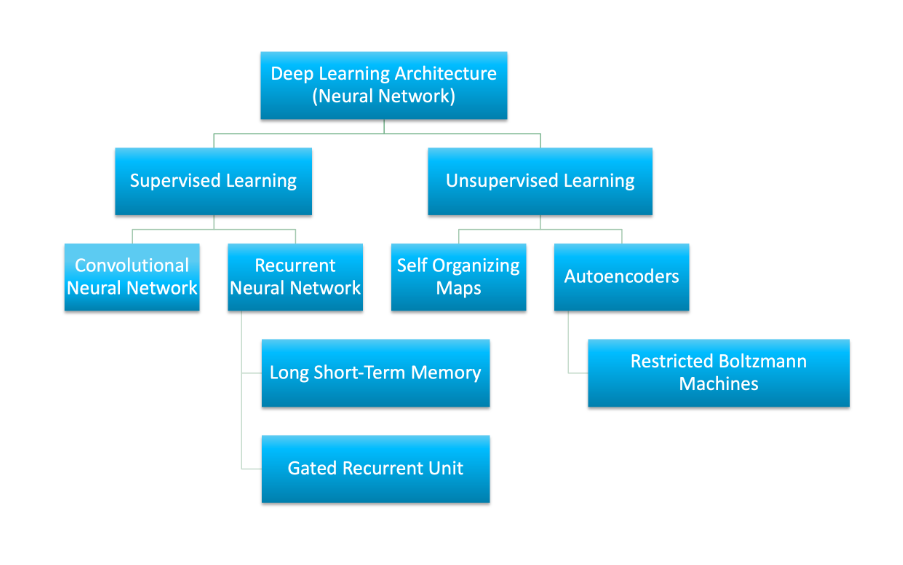
\includegraphics[width=1\textwidth]{DeepLearning_Arch.PNG}
    \caption{Deep learning architectures \cite{madhavan2017deep}}
\end{figure}
\begin{itemize}
    \item \textbf{Supervised deep learning: }
    \href{https://developer.ibm.com/articles/cc-machine-learning-deep-learning-architectures/}{\textcolor{blue}{Source}}
    Supervised learning refers to the problem space wherein the target to be predicted is clearly labeled within the data that is used for training.
    \begin{itemize}
        \item \textbf{Convolutional neural networks: } A CNN is a multilayer neural network used for image processing, inspired by the animal visual cortex. It was first created by Yann LeCun for recognizing handwritten characters. Early layers detect basic features, while subsequent layers combine these features to extract higher-level attributes of the input image. The LeNet CNN architecture performs feature extraction and classification through multiple layers, including convolutional and pooling layers, a fully connected multilayer perceptron, and an output layer. 
        \begin{figure}[H]
            \centering
            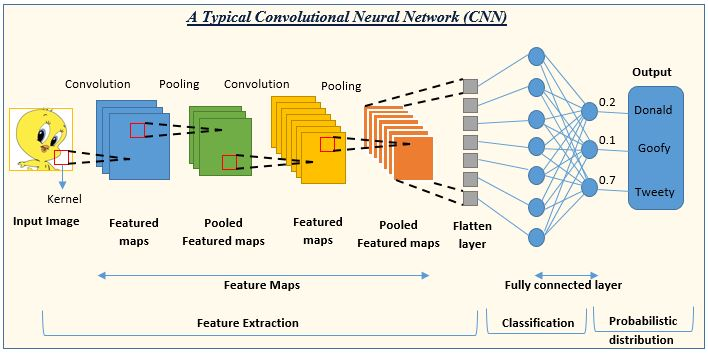
\includegraphics[width=0.8\linewidth]{tex/img/CNN.jpeg}
            \caption{Convolutional Neural Network \protect\href{https://www.analyticsvidhya.com/blog/2022/01/convolutional-neural-network-an-overview/}{\textcolor{blue}{source}} }
            \label{fig:CNN}
        \end{figure}
        The network is trained through back-propagation. A Convolutional Neural Network (CNN) is a highly effective multilayer neural network that was inspired by the visual cortex of animals. It is primarily used for image processing applications. The first-ever CNN was created by Yann LeCun, which revolutionized the recognition of handwritten characters such as postal codes.
        
        With its deep network architecture, CNN can detect basic features, such as edges, through its initial layers and then combine these features to extract higher-level attributes of the input image.
        
        The LeNet CNN architecture, consisting of multiple layers that perform feature extraction and classification, is a prime example of CNN's effectiveness. It includes convolutional and pooling layers, a fully connected multilayer perceptron, and an output layer that identifies features of the image. The network is trained through back-propagation, making it an even more efficient tool. \cite{alzubaidi2021review} \cite{ansari2020building}
        
        \item  \textbf{The Gated Recurrent Unit (GRU) networks} In 2014, a simplification of the LSTM was introduced called the gated recurrent unit. This model has two gates, getting rid of the output gate present in the LSTM model. These gates are an update gate and a reset gate. The update gate indicates how much of the previous cell contents to maintain. The reset gate defines how to incorporate the new input with the previous cell contents. A GRU can model a standard RNN simply by setting the reset gate to 1 and the update gate to 0. \cite{madhavan2017deep}
        
        \begin{figure}[H]
            \centering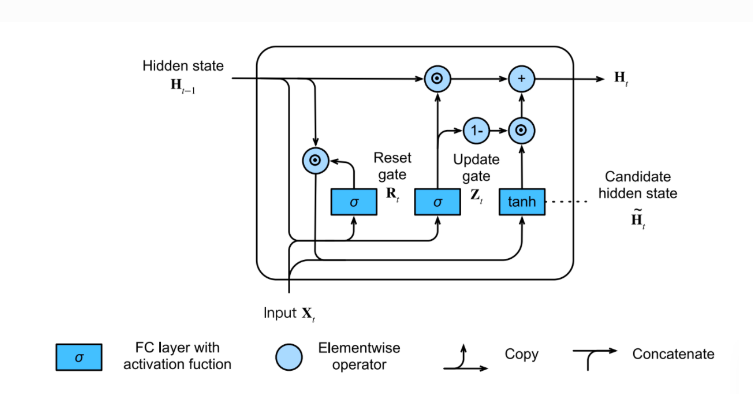
\includegraphics[width=1\textwidth]{GRU_layers.PNG}
            \caption{GRU networks}
        \end{figure}
        The GRU is simpler than the LSTM, can be trained more quickly, and can be more efficient in its execution. However, the LSTM can be more expressive and with more data can lead to better results.
    \end{itemize}

     \item \textbf{Recurrent Neural Network (RNN): } RNN is the neural network with hidden state, which captures the historical information up to the current timestep. Because the hidden state of the current state uses the same definition as that in the previous timestep, which means the computation is recurrent, hence it is called recurrent neural network.

     The RNN is one of the foundational network architectures from which other deep learning architectures are built. The primary difference between a typical multilayer network and a recurrent network is that rather than completely feed-forward connections, a recurrent network might have connections that feed back into prior layers (or into the same layer). This feedback allows RNNs to maintain memory of past inputs and model problems in time.

    RNNs consist of a rich set of architectures (we'll look at one popular topology called LSTM next). The key differentiator is feedback within the network, which could manifest itself from a hidden layer, the output layer, or some combination thereof.
    RNNs can be unfolded over time and trained using standard back-propagation or a variant called back-propagation through time (BPTT).  \cite{sherstinsky2020fundamentals}\\
    \begin{figure}[H]
        \centering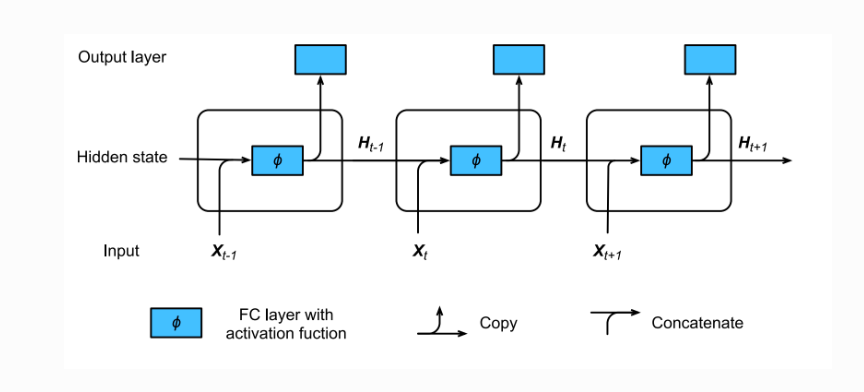
\includegraphics[width=0.8\textwidth]{RNN.PNG}
        \caption{Recurrent Neural Network}
    \end{figure}
    \item \textbf{Gated Recurrent Unit (GRU) Layer: } GRU supports: \\
    \textbf{hidden gate} the gating of hidden state, \\
    \textbf{Reset gate} controls how much of the previous hidden state we might still want to remember.\\
    \textbf{Update gate} controls how much of current hidden state is just a copy of the previous state
    The structure and math are as follow:
    \begin{figure}[H]
        \centering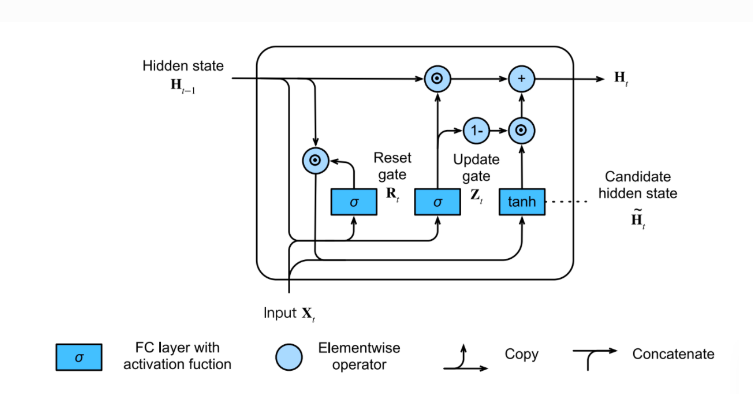
\includegraphics[width=0.8\textwidth]{GRU_layers.PNG}
        \caption{Gated Recurrent Unit}
    \end{figure}
    \item \textbf{Long short-term memory (LSTM): } Long Short-Term Memory (LSTM) is a type of recurrent neural network (RNN) architecture designed to address the vanishing gradient problem that can occur in traditional RNNs. LSTMs are well-suited for tasks that involve sequences of data, such as time series analysis, natural language processing, speech recognition, and more.

    The key feature of LSTMs is their ability to capture and remember long-term dependencies in sequential data while avoiding the vanishing gradient problem, which can hinder the training of RNNs over long sequences. \cite{alzubaidi2021review} \cite{madhavan2017deep}
    
    Here are the main components and features of an LSTM:
    
    \textbf{Cell State (Ct):}
    
    The cell state is the long-term memory of the LSTM. It runs straight down the entire chain of the LSTM, with only some minor linear interactions. It acts as a conveyor belt that runs through the entire sequence, and information can be added or removed to and from the cell state.\\
    
    \textbf{Hidden State (ht):}\\
    
    The hidden state is the short-term memory of the LSTM. It is responsible for capturing and remembering short-term dependencies in the sequence. The hidden state at each time step depends on both the current input and the previous hidden state.\\
    \textbf{Input Gate: } 
    The input gate determines how much of the new information from the current input should be added to the cell state. It involves a sigmoid activation function, which decides which values should be updated (values close to 1) and which should be ignored (values close to 0).\\
    \textbf{Forget Gate:}
    
    The forget gate decides which information from the cell state should be discarded. It considers the previous hidden state and the current input to decide which parts of the cell state are no longer relevant. It involves a sigmoid activation function to output values between 0 and 1.\\
    \textbf{Cell State Update}:
    The input gate and forget gate jointly determine the update to the cell state. The input gate decides what new information to store in the cell state, and the forget gate decides what information to remove.\\
    \textbf{Output Gate:}
    
    The output gate decides what the next hidden state should be. It involves a sigmoid activation function and a tanh activation function. The sigmoid decides which parts of the cell state to output, and the tanh creates a vector of new candidate values to be added to the hidden state.
    \href{https://ml-cheatsheet.readthedocs.io/en/latest/layers.html#lstm}{Layers}
    \begin{figure}[H]
        \centering
        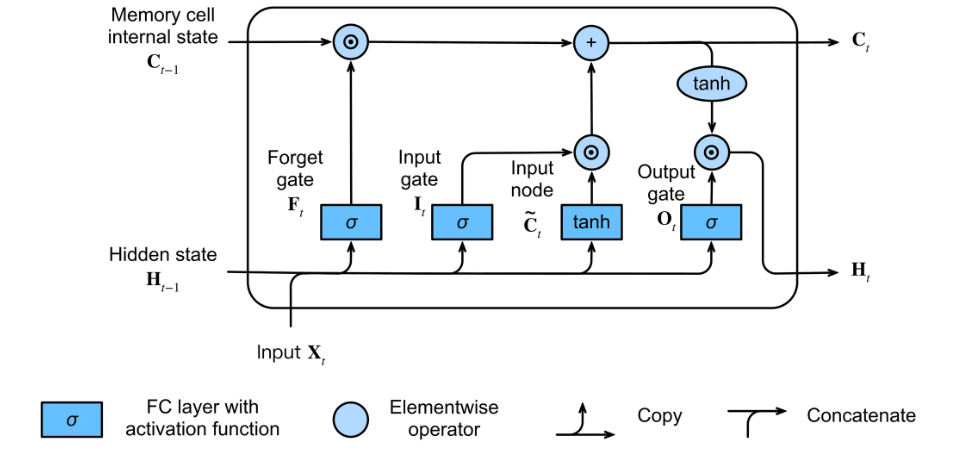
\includegraphics[width=0.8\linewidth]{tex/img/LSTM_layer.PNG}
        \caption{Long short-term memory \protect\href{https://link.springer.com/article/10.1007/s10586-022-03707-y/figures/6}{\textcolor{blue}{source}}}
        \label{fig:LSTM_layer}
    \end{figure}
    \end{itemize}

\end{itemize}

\subsubsection{Section Unsupervised learning}

Unsupervised learning refers to the problem space wherein there is no target label within the data that is used for training, and there are several unsupervised architectures.\cite{coates2011analysis}
\begin{itemize}
    \item \textbf{Self-organized maps: } Self-organized map (SOM) was invented by Dr. Teuvo Kohonen in 1982 and was popularly known as the Kohonen map. SOM is an unsupervised neural network that creates clusters of the input data set by reducing the dimensionality of the input. SOMs vary from the traditional artificial neural network in quite a few ways. \cite{alzubaidi2021review}, \cite{madhavan2017deep}

    \begin{figure}[H]
        \centering
        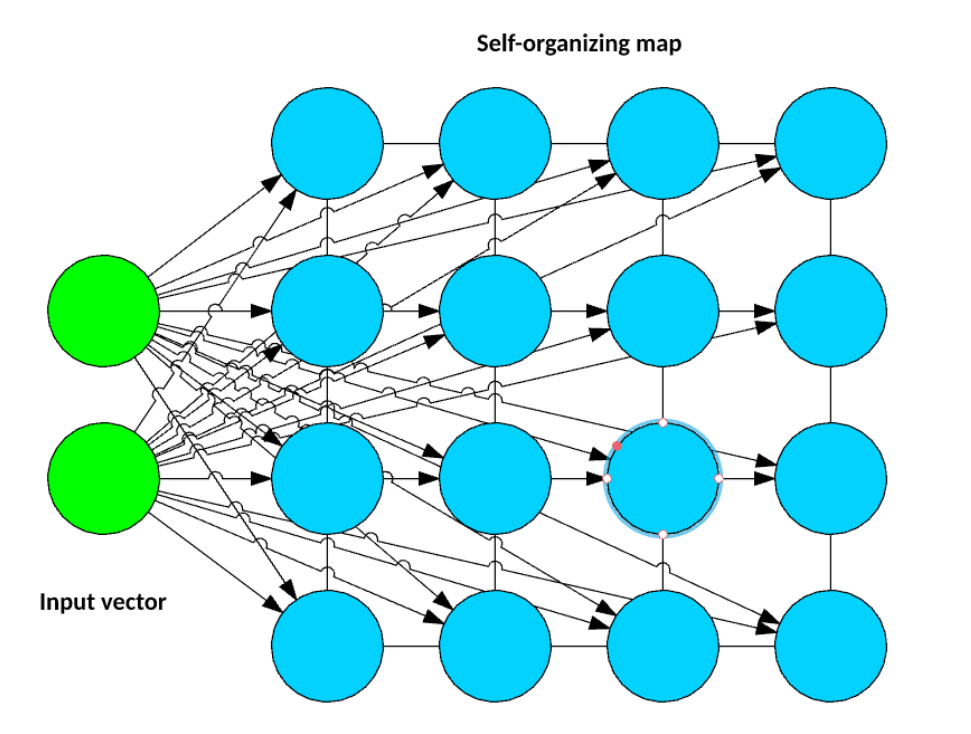
\includegraphics[width=0.5\textwidth]{Self_organizingMap.PNG}
        \caption{Self-organized map (SOM)}
        \label{fig:Self-organized map (SOM)}
    \end{figure}
    \textbf{Example applications:} Dimensionality reduction, clustering high-dimensional inputs to 2-dimensional output, radiant grade result, and cluster visualization
    \item \textbf{Autoencoders: } This variant of an ANN is composed of 3 layers: input, hidden, and output layers.
    First, the input layer is encoded into the hidden layer using an appropriate encoding function. The number of nodes in the hidden layer is much less than the number of nodes in the input layer. This hidden layer contains the compressed representation of the original input. The output layer aims to reconstruct the input layer by using a decoder function.
    
    \begin{figure}[H]
        \centering
        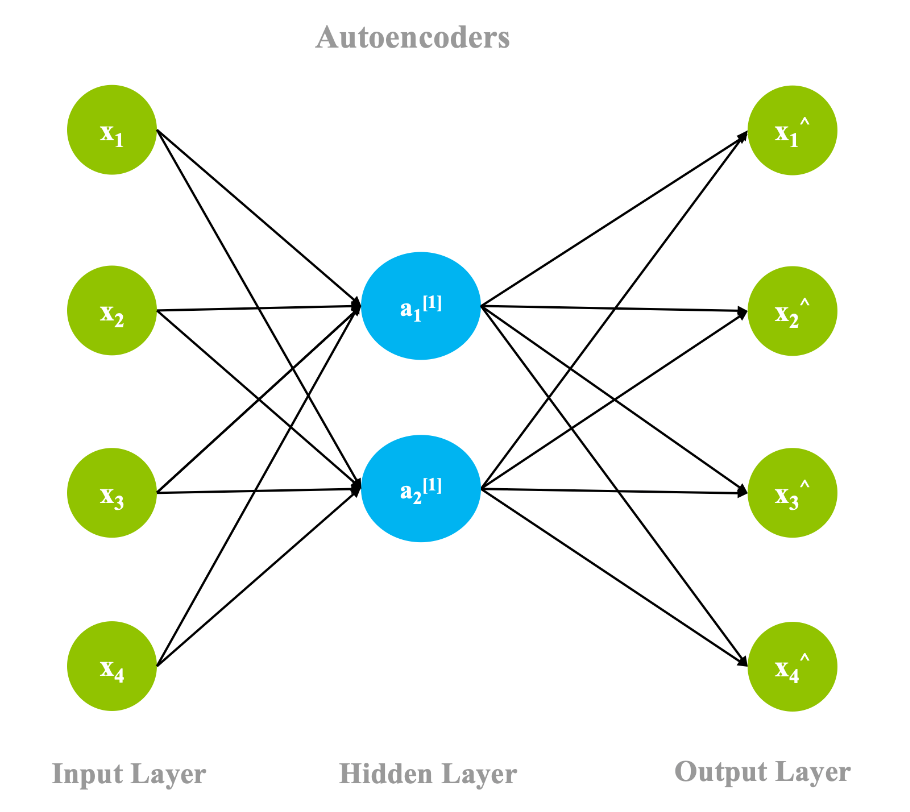
\includegraphics[width=0.7\linewidth]{tex/img/Autoencoders.PNG}
        \caption{Autoencoders}
        \label{fig:Autoencoders}
    \end{figure}
    During the training phase, the difference between the input and the output layers is calculated using an error function, and the weights are adjusted to minimize the error. \\ 
    \textbf{Example applications:} Dimensionality reduction, data interpolation, and data compression/decompression.\\ 
    \item \textbf{Restricted Boltzmann Machines: } An RBM is a two-layered neural network. The layers are input and hidden layers. As shown in the following figure \ref{fig:Restricted Boltzmann Machines}, in RBMs, every node in a hidden layer is connected to every node in a visible layer. In a traditional Boltzmann machine, nodes within the input and hidden layers are also connected. Due to computational complexity, nodes within a layer are not connected in a restricted Boltzmann machine.
    
    \begin{figure}[H]
        \centering
        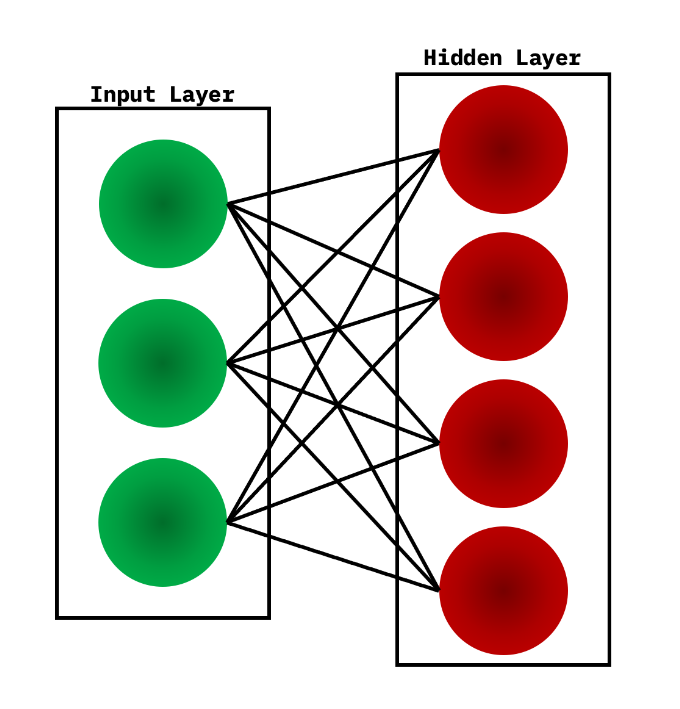
\includegraphics[width=0.6\textwidth]{RestrictedBoltzmannMachines.PNG}
        \caption{Restricted Boltzmann Machines}
        \label{fig:Restricted Boltzmann Machines}
    \end{figure}
    During the training phase, RBMs calculate the probability distribution of the training set using a stochastic approach. When the training begins, each neuron gets activated at random. Also, the model contains respective hidden and visible biases. While the hidden bias is used in the forward pass to build the activation, the visible bias helps in reconstructing the input. Because in an RBM the reconstructed input is always different from the original input, they are also known as generative models.
    Also, because of the built-in randomness, the same predictions result in different outputs. In fact, this is the most significant difference from an autoencoder, which is a deterministic model. \cite{madhavan2017deep} \cite{alzubaidi2021review} \\
    \textbf{Example applications:} Dimensionality reduction and collaborative filtering.\\
    \item \textbf{Deep belief networks: } The DBN is a multilayer network (typically deep and including many hidden layers) in which each pair of connected layers is an RBM. In this way, a DBN is represented as a stack of RBMs.
    In the DBN, the input layer represents the raw sensory inputs, and each hidden layer learns abstract representations of this input. The output layer, treated differently, is responsible for network classification during training. Training occurs in two steps: unsupervised pretraining and supervised fine-tuning. \cite{sohn2021deep}, \cite{coates2011analysis}
    
    \begin{figure}[H]
        \centering
        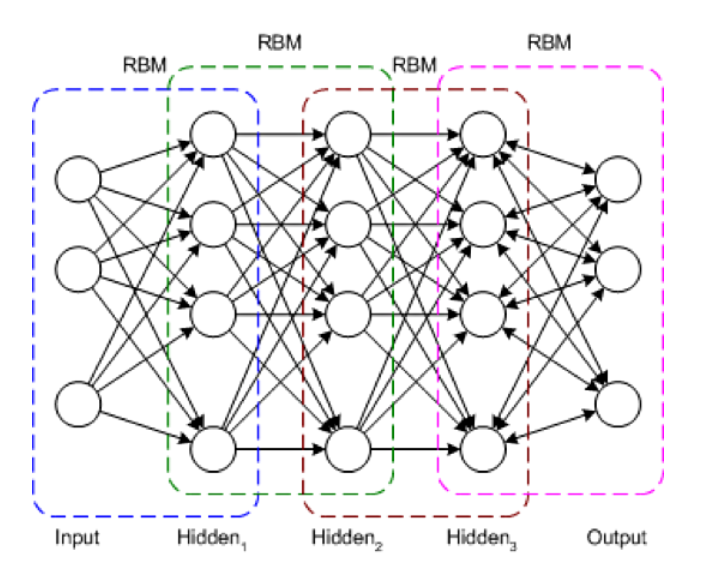
\includegraphics[width=0.7\textwidth]{DeepBelief_Networks.PNG}
        \caption{Deep belief networks architecture}
        \label{fig:Deep belief networks}
    \end{figure}
    In unsupervised pretraining, each RBM is trained to reconstruct its input (for example, the first RBM reconstructs the input layer to the first hidden layer). The next RBM is trained similarly, but the first hidden layer is treated as the input (or visible) layer, and the RBM is trained by using the outputs of the first hidden layer as the inputs. This process continues until each layer is pretrained. When the pretraining is complete, fine-tuning begins. In this phase, the output nodes are given labels to give them meaning (what they represent in the context of the network). Full network training is then applied by using either gradient descent learning or back-propagation to complete the training process. \\
    \textbf{Example applications: }Image recognition, information retrieval, natural language understanding, and failure prediction. \\
    \item \textbf{Deep stacking networks: } It is also called a deep convex network. A DSN is different from traditional deep learning frameworks in that, although it consists of a deep network, it's actually a deep set of individual networks, each with its own hidden layers.
    This architecture is a response to one of the problems with deep learning: the complexity of training. Each layer in a deep learning architecture exponentially increases the complexity of training, so the DSN views training not as a single problem but as a set of individual training problems.
    The DSN consists of a set of modules, each of which is a subnetwork in the overall hierarchy of the DSN. In one instance of this architecture, three modules are created for the DSN. Each module consists of an input layer, a single hidden layer, and an output layer. Modules are stacked one on top of another, where the inputs of a module consist of the prior layer outputs and the original input vector. This layering allows the overall network to learn more complex classifications than would be possible given a single module. \cite{deng2014tutorial}, \cite{madhavan2017deep}
    
    \begin{figure}[H]
        \centering
        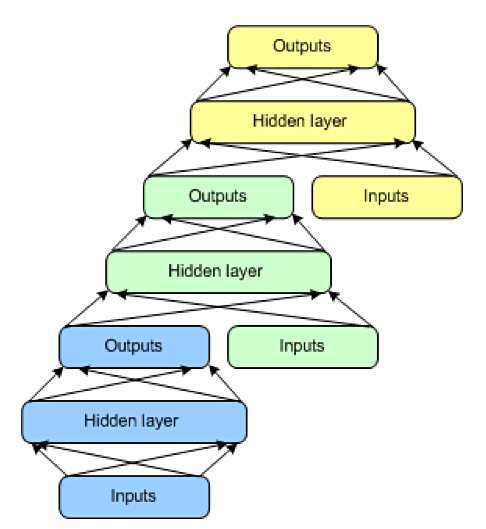
\includegraphics[width=0.5\textwidth]{DeepStackNetworks.PNG}
        \caption{Deep stacking networks architecture}
        \label{fig:Deep stacking networks}
    \end{figure}
    \textbf{Example applications:} Information retrieval and continuous speech recognition
    

\end{itemize}
